% Chapter 3
\chapter{CƠ SỞ LÝ THUYẾT VÀ CÔNG NGHỆ NỀN TẢNG}
\label{Chapter3}

Chương này xây dựng cơ sở lý thuyết cho sáu thành phần: Federated Learning, tấn công poisoning/backdoor, Digital Twin, mô hình sinh dữ liệu bảng, mô hình IDS, và bộ dữ liệu thực nghiệm.

\section{Cơ sở lý thuyết Federated Learning}
Federated Learning (FL) là nền tảng mà DT-Guard được xây dựng trên đó. Phần này phân tích bài toán tối ưu phân tán, thuật toán FedAvg, đặc thù dữ liệu Non-IID, và cơ chế Weighted Cross-Entropy Loss để xử lý mất cân bằng lớp.

\subsection{Bài toán tối ưu phân tán trong FL}
Bài toán FL được xây dựng dựa trên bài toán tối ưu hóa phân tán. Giả sử có $N$ clients tham gia vào quá trình huấn luyện. Mỗi client $i$ có dữ liệu cục bộ $D_{i}$ với $n_{i}$ mẫu. Mục tiêu là tìm tham số mô hình tối ưu $\mathbf{w}^{*}$ giúp tối thiểu hàm mất mát tổng thể $F(\mathbf{w})$.

Hàm mất mát tổng thể được tính là trung bình có trọng số của các hàm mất mát cục bộ từ tất cả clients, trong đó trọng số của mỗi client tỷ lệ với số lượng mẫu dữ liệu họ sở hữu. Điều này đảm bảo rằng client có nhiều dữ liệu hơn có ảnh hưởng lớn hơn đến mô hình toàn cục.

Bài toán này có nhiều thách thức trong môi trường phân tán: (1) Server không có quyền truy cập dữ liệu thô $D_{i}$ của bất kỳ client nào; (2) Giao tiếp giữa server và clients bị hạn chế về băng thông; (3) Số lượng và cấu hình của clients có thể thay đổi theo thời gian; (4) Một số clients có thể độc hại hoặc không hợp tác.

\subsection{Thuật toán FedAvg}
FedAvg (Federated Averaging) là thuật toán tổng hợp mặc định trong Federated Learning, được giới thiệu bởi McMahan và cộng sự năm 2017 {[}9{]}. Thuật toán hoạt động theo nhiều round (vòng lặp), mỗi round bao gồm các bước sau:

\textbf{Bước 1: Khởi tạo và phân phối.} Server khởi tạo tham số mô hình $\mathbf{w}^{(0)}$ (có thể ngẫu nhiên hoặc từ kiến thức sẵn có) và gửi cho tất cả clients tham gia.

\textbf{Bước 2: Huấn luyện cục bộ.} Mỗi client i nhận $\mathbf{w}^{(t-1)}$ từ server, sau đó huấn luyện mô hình cục bộ trên dữ liệu riêng $D_{i}$ trong một số epoch nhất định E (local epochs). Quá trình huấn luyện cục bộ sử dụng thuật toán tối ưu hóa như Stochastic Gradient Descent (SGD) để cập nhật tham số từ $\mathbf{w}^{(t-1)}$ thành $\mathbf{w}_{i}^{(t)}$.

\textbf{Bước 3: Gửi bản cập nhật về server.} Sau khi hoàn thành huấn luyện cục bộ, mỗi client gửi tham số mô hình $\mathbf{w}_{i}^{(t)}$ về server. Trong một số biến thể, client có thể gửi gradient cập nhật thay vì tham số đầy đủ.

\textbf{Bước 4: Tổng hợp tại server.} Server nhận tất cả bản cập nhật từ clients và tổng hợp thành tham số mô hình toàn cục mới $\mathbf{w}^{(t)}$ bằng cách lấy trung bình có trọng số. Trọng số của mỗi client tỷ lệ với số lượng mẫu dữ liệu họ có, client có nhiều dữ liệu hơn có ảnh hưởng lớn hơn đến mô hình toàn cục. Cụ thể, tham số mới được tính bằng tổng của (tham số mỗi client $\times$ trọng số tương ứng) chia cho tổng trọng số.

\textbf{Bước 5: Lặp lại.} Server gửi $\mathbf{w}^{(t)}$ về cho tất cả clients và quá trình lặp lại từ Bước 2 cho đến khi mô hình hội tụ đến điểm tối ưu hoặc đạt tiêu chí dừng được định nghĩa trước.

Thuật toán FedAvg hoạt động hiệu quả khi dữ liệu được phân phối IID (Independent and Identically Distributed) giữa các clients. Tuy nhiên, trong môi trường IoT thực tế, dữ liệu thường có đặc tính Non-IID nghiêm trọng, dẫn đến các thách thức về hội tụ và hiệu năng.

\subsection{Dữ liệu Non-IID trong FL}
Dữ liệu Non-IID (Non-Independent and Identically Distributed) là đặc thù quan trọng nhất của FL trong môi trường IoT. Non-IID có thể được phân loại thành ba dạng skew chính:

\textbf{Label skew (sai lệch nhãn):} Các clients có phân bố nhãn khác nhau. Ví dụ, một client có chủ yếu lưu lượng bình thường, trong khi client khác có chủ yếu lưu lượng tấn công DDoS. Trong ngữ cảnh IoT IDS, label skew xảy ra vì các thiết bị IoT có thể được triển khai trong các môi trường khác nhau (nhà thông minh, bệnh viện, nhà máy), mỗi môi trường có mô hình tấn công đặc thù.

\textbf{Quantity skew (sai lệch số lượng):} Các clients có số lượng mẫu khác nhau. Một số clients có thể có hàng triệu mẫu lưu lượng mạng, trong khi clients khác chỉ có hàng nghìn mẫu. Điều này dẫn đến việc clients có nhiều dữ liệu có ảnh hưởng lớn hơn đến mô hình toàn cục thông qua cơ chế gán trọng số của FedAvg.

\textbf{Feature skew (sai lệch đặc trưng):} Các clients có cùng nhãn nhưng phân bố đặc trưng khác nhau. Ví dụ, lưu lượng bình thường trong mạng bệnh viện có thể có đặc trưng khác với lưu lượng bình thường trong mạng nhà thông minh do giao thức, cấu trúc mạng, và hành vi người dùng khác nhau.

Để mô phỏng đặc tính Non-IID trong thực nghiệm, phương pháp phổ biến là sử dụng phân phối Dirichlet. Tham số $\alpha$ điều khiển mức độ Non-IID: $\alpha$ càng nhỏ thì sự chênh lệch phân bố nhãn giữa các client càng lớn. Mỗi client nhận một phân phối nhãn được sinh ngẫu nhiên theo Dirichlet, sau đó được gán mẫu tương ứng theo phân phối đó.

Trong ngữ cảnh IoT IDS, Non-IID tạo ra hai thách thức chính cho các phương pháp phòng thủ: (1) Clients lành tính có tham số lệch xa nhau do dữ liệu khác nhau, khiến các bộ lọc dựa trên khoảng cách tham số dễ nhầm lẫn với client độc hại; (2) Các client có dữ liệu ít đại diện cho không gian toàn bộ có thể gửi cập nhật "bất thường" nhưng thực sự hữu ích.

\subsection{Weighted Cross-Entropy Loss cho mất cân bằng lớp}
\label{subsec:wce_loss}
Trong bộ dữ liệu IoT IDS như CIC-IoT-2023 và ToN-IoT, vấn đề mất cân bằng lớp nghiêm trọng: lưu lượng bình thường thường chiếm 50--60\% dữ liệu, trong khi một số lớp tấn công chỉ chiếm 1--2\%. Mất cân bằng này khiến mô hình có xu hướng thiên lệch về lớp chiếm đa số, dẫn đến hiệu năng kém trên các lớp thiểu số.

Cross-Entropy Loss truyền thống đo sự khác biệt giữa phân phối xác suất dự đoán và nhãn thật. Khi tính loss trung bình trên tất cả mẫu, mỗi mẫu đóng góp như nhau, không phân biệt mẫu thuộc lớp nào. Trong ngữ cảnh mất cân bằng, lớp chiếm đa số (ví dụ: bình thường, 60\% dữ liệu) sẽ chi phối tổng loss, khiến mô hình tối ưu hóa cho lớp này mà bỏ qua lớp thiểu số (ví dụ: tấn công Backdoor, chỉ 1\% dữ liệu).

Để xử lý vấn đề này, Weighted Cross-Entropy Loss gán trọng số cho từng lớp ngược lại với tần suất xuất hiện: lớp càng hiếm thì trọng số càng lớn. Cụ thể, trọng số cho một lớp được tính bằng tổng số mẫu chia cho (số lớp $\times$ số mẫu của lớp đó). Ví dụ, nếu lớp bình thường chiếm 60\% và lớp tấn công chỉ chiếm 1\%, thì trọng số của lớp tấn công lớn gấp khoảng 60 lần. Khi đó, mô hình "phạt nặng" hơn khi phân loại sai lớp hiếm, buộc phải học cả các mẫu tấn công ít xuất hiện.

Trong DT-Guard, Weighted Cross-Entropy Loss được sử dụng trong cả quá trình huấn luyện cục bộ trên clients và trong việc đánh giá hiệu năng IDS trên challenge data.

\section{Cơ sở lý thuyết các tấn công poisoning và backdoor}
Mục 2.4 đã trình bày tổng quan về năm loại tấn công poisoning, backdoor và vấn đề free-rider trong FL. Phần này đi sâu vào cơ chế kỹ thuật của từng tấn công để làm cơ sở cho thiết kế pipeline phòng thủ trong Chương 4.

\subsection{Tấn công LIE (A Little Is Enough)}
Như đã giới thiệu ở Mục 2.4.2, LIE {[}1{]} tạo tham số độc hại nằm trong vùng phân phối thống kê bình thường. Về mặt kỹ thuật, với mỗi chiều tham số, attacker tính giá trị trung bình và độ lệch chuẩn từ các bản cập nhật lành tính, sau đó tạo tham số độc hại bằng cách cộng thêm một lượng nhỏ (được điều chỉnh bởi tham số z) vào giá trị trung bình. Tham số z được chọn sao cho tham số độc hại vẫn nằm trong vùng tin cậy của phân phối, khiến các bộ lọc dựa trên khoảng cách (Krum, Median, Trimmed Mean) không thể phát hiện vì tham số độc hại không phải là outlier.

\subsection{Tấn công Min-Max và Min-Sum}
Min-Max và Min-Sum {[}15{]} là hai tấn công tối ưu hóa ảnh hưởng đầu độc dưới ràng buộc khoảng cách, được giới thiệu bởi Shejwalkar và Houmansadr năm 2021.

Min-Max attack giải bài toán: tìm bản cập nhật độc hại sao cho ảnh hưởng lên mô hình toàn cục là lớn nhất, đồng thời khoảng cách từ bản cập nhật độc hại đến mỗi bản cập nhật lành tính không vượt quá một ngưỡng $\varepsilon$ cho trước. Bài toán này thường được giải bằng phương pháp binary search kết hợp projected gradient ascent, mỗi bước tăng ảnh hưởng nhưng chiếu lại vào vùng hợp lệ (khoảng cách $\leq$ $\varepsilon)$. Kết quả là bản cập nhật độc hại có ảnh hưởng tối đa mà vẫn vượt qua được các bộ lọc khoảng cách.

Min-Sum attack có chiến lược tương tự nhưng kiểm soát tổng khoảng cách từ bản cập nhật độc hại đến tất cả update lành tính, thay vì khoảng cách tối đa đến từng update riêng lẻ. Điều này cho phép attacker linh hoạt hơn trong việc phân bổ "ngân sách khoảng cách."

Cả hai đều nhắm vào các phương pháp phòng thủ dựa trên khoảng cách như Krum (chọn update có tổng khoảng cách nhỏ nhất) và GeoMed (tìm geometric median), vì bản cập nhật độc hại luôn nằm trong vùng khoảng cách cho phép.

\subsection{Tấn công MPAF}
MPAF {[}3{]} (Model Poisoning Attacks based on Fake clients) là tấn công được thiết kế đặc biệt để phá vỡ giả định honest majority (giả định rằng đa số client là lành tính) mà nhiều phương pháp phòng thủ dựa vào.

Cơ chế thực hiện như sau: attacker tạo nhiều client ảo (ví dụ: 5--10 fake clients khi tổng số client là 20), mỗi fake client gửi một bản cập nhật độc hại tương tự nhau. Kết quả là các bản cập nhật độc hại chiếm đa số trong tập update, khiến các phương pháp phòng thủ không thể loại bỏ. Cụ thể: Krum chỉ chọn 1 update và có thể chọn update độc hại nếu đa số là độc hại; Median/Trimmed Mean cắt tỷ lệ $\beta$ cực trị nhưng nếu tỷ lệ độc hại vượt $\beta$ thì không thể loại bỏ hết; phương pháp phân cụm dựa trên cosine distance bị nhầm vì cụm độc hại chiếm đa số.

\subsection{Tấn công Backdoor}
Như đã phân tích ở Mục 2.4.2, backdoor attack chèn trigger pattern vào dữ liệu để mô hình phân loại sai khi gặp trigger. Về mặt hàm mất mát, client độc hại tối thiểu hóa đồng thời hai thành phần: sai số trên dữ liệu bình thường và sai số trên dữ liệu có chứa trigger. Một tham số cân bằng điều chỉnh mức độ ưu tiên giữa hai thành phần: tham số này càng lớn thì mô hình càng tập trung vào việc học backdoor, làm cho trigger phát huy tác dụng mạnh hơn khi gặp mẫu chứa trigger.

\subsection{Free-rider problem}
Free-rider sao chép mô hình toàn cục kèm nhiễu nhỏ thay vì huấn luyện (xem Mục 2.4.1). Cụ thể, free-rider nhận mô hình toàn cục từ server rồi thêm một lượng nhiễu rất nhỏ vào tham số và gửi lại, thay vì thực hiện huấn luyện trên dữ liệu riêng. Vấn đề nghiêm trọng là các phương pháp phòng thủ dựa trên khoảng cách tham số (Trust Score trong DT-BFL {[}5{]}, PoC trong PPSG {[}22{]}) đánh giá free-rider "đáng tin" nhất vì tham số của free-rider gần giống mô hình toàn cục nhất.

\section{Cơ sở lý thuyết Digital Twin}
Để DT-Guard có thể "kiểm tra" mô hình client trước khi tin tưởng, cần làm rõ Digital Twin (DT) là gì, gồm những thành phần nào và vì sao nó lại phù hợp với vai trò sandbox phía server. Các nội dung dưới đây làm rõ những điểm này, đồng thời đối sánh hai cách tiếp cận: kiểm chứng hành vi chủ động và phân tích tham số một cách thụ động.

\subsection{Mô hình khái niệm Digital Twin}
Digital Twin (DT) là một bản sao số của một thực thể vật lý được kết nối liên tục để phản ánh trạng thái và hành vi của thực thể đó. Khái niệm này đã phát triển từ những nghiên cứu ban đầu trong lĩnh vực hàng không vũ trụ (NASA) và sau đó được mở rộng sang các lĩnh vực như sản xuất, đô thị thông minh, và IoT.

\textbf{Thành phần cơ bản của Digital Twin} bao gồm bốn thành phần chính:

\textbf{(1) Physical Entity (PE)} là thực thể vật lý cần sao chép (ví dụ: thiết bị IoT, hệ thống sản xuất, hoặc toàn bộ mạng IoT). PE có trạng thái và hành vi có thể được quan sát và đo lường.

\textbf{(2) Digital Model (DM)} là bản sao số phản ánh các đặc trưng quan trọng của PE. DM không nhất thiết phải sao chép đầy đủ mọi chi tiết của PE, chỉ cần phản ánh các đặc trưng liên quan đến ứng dụng cụ thể. Trong ngữ cảnh FL-IDS, DM là mô hình máy học phản ánh hành vi của client trên dữ liệu mạng.

\textbf{(3) Data Connection (DC)} là cơ chế kết nối giữa PE và DM cho phép trao đổi dữ liệu hai chiều. DC thu thập dữ liệu telemetry từ PE về DM để cập nhật trạng thái, và gửi lệnh điều khiển hoặc tham số từ DM về PE để điều khiển hành vi.

\textbf{(4) Services (S)} là các dịch vụ được xây dựng trên nền tảng DM để thực hiện các nhiệm vụ như mô phỏng, dự báo, tối ưu hóa, và kiểm thử.

\textbf{Vòng đời Digital Twin} gồm năm giai đoạn:

\textbf{Giai đoạn 1: Tạo (Create)}: Khởi tạo Digital Model dựa trên kiến thức về Physical Entity. Có thể sử dụng dữ liệu lịch sử, mô hình vật lý, hoặc các kỹ thuật machine learning.

\textbf{Giai đoạn 2: Kết nối (Connect)}: Thiết lập Data Connection giữa Physical Entity và Digital Model, cho phép trao đổi dữ liệu hai chiều.

\textbf{Giai đoạn 3: Mô phỏng (Simulate)}: Sử dụng Digital Model để mô phỏng hành vi của Physical Entity trong các điều kiện khác nhau hoặc dự báo trạng thái trong tương lai.

\textbf{Giai đoạn 4: Phân tích (Analyze)}: Phân tích kết quả mô phỏng để phát hiện bất thường, xác định nguyên nhân, hoặc tìm kiếm cơ hội cải thiện.

\textbf{Giai đoạn 5: Tối ưu hóa và hành động (Optimize \& Actuate)}: Tìm các tham số vận hành tối ưu cho Physical Entity và áp dụng các hành động từ hệ thống kỹ thuật số về thiết bị vật lý.

\begin{figure}[H]
    \centering
    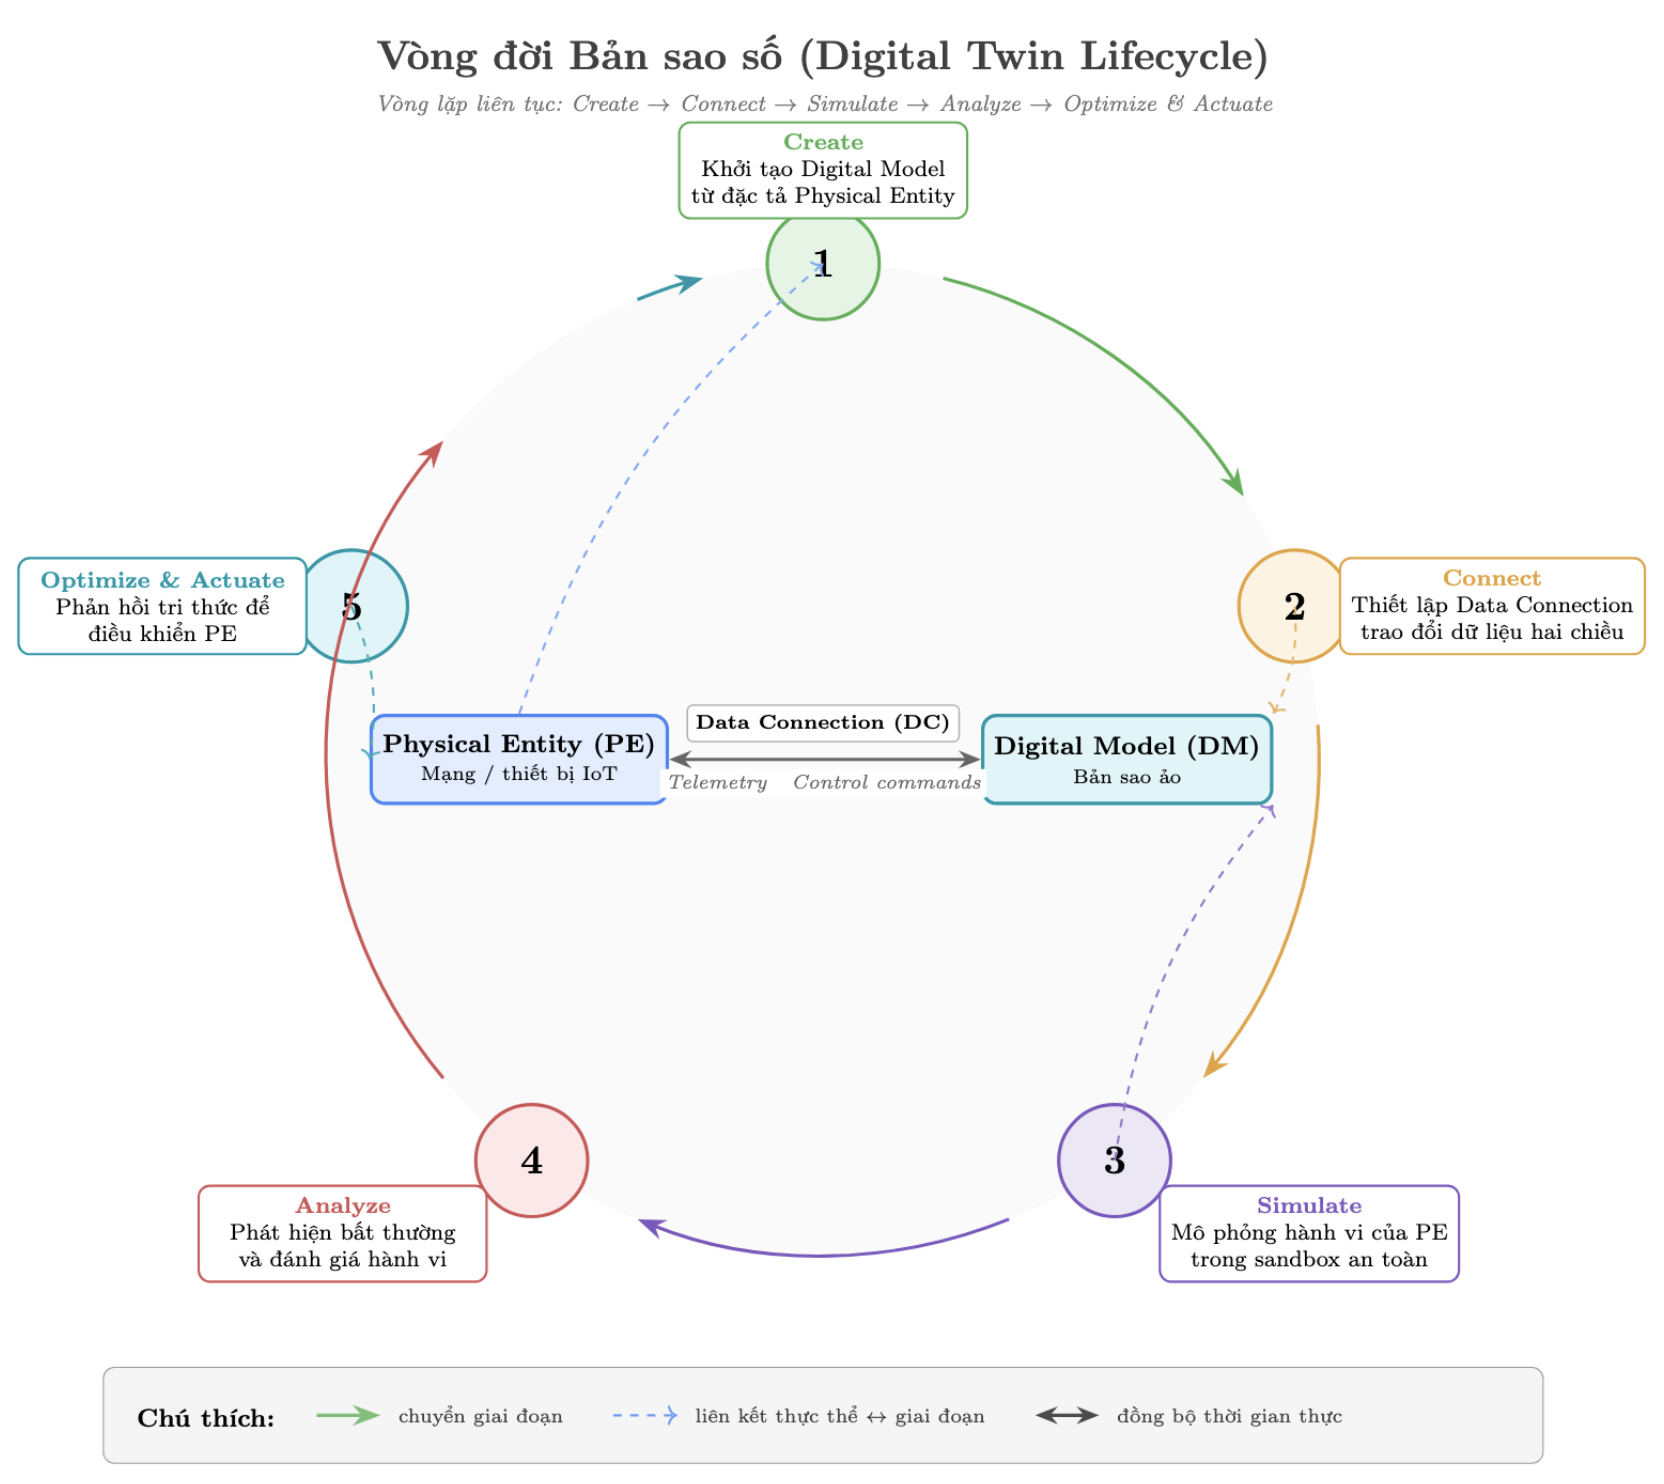
\includegraphics[width=0.85\linewidth]{Figures/fig_3_1_vong_doi_digital_twin.png}
    \caption{Vòng đời Digital Twin}
\end{figure}

Trong ngữ cảnh IoT, Digital Twin có nhiều ứng dụng như simulation (mô phỏng kịch bản khác nhau trên DT để dự báo hành vi trong tương lai hoặc kiểm thử chiến lược mới), optimization (tìm các tham số vận hành tối ưu cho thiết bị vật lý), anomaly detection (so sánh giữa trạng thái dự báo của DT và trạng thái thực tế của PE để phát hiện sai lệch), testing (kiểm thử hành vi hoặc chiến lược mới trong môi trường an toàn), và actuation (áp dụng các điều khiển hoặc hành động từ hệ thống kỹ thuật số về thiết bị vật lý).

\subsection{Server-side DT cho behavioral testing}
Trong DT-Guard, Digital Twin có chức năng khác biệt so với các ứng dụng DT truyền thống. Thay vì mirror một thiết bị vật lý cụ thể, Digital Twin trong DT-Guard là một môi trường kiểm thử (sandbox) tại server để chủ động kiểm chứng hành vi của từng mô hình cục bộ từ clients.

Sandbox isolation là một khía cạnh quan trọng của Digital Twin trong DT-Guard. Sandbox được tách biệt từ FL Server chính, có nghĩa là hành vi độc hại của một client không ảnh hưởng trực tiếp đến server hay các clients khác. Khi server nhận bản cập nhật từ một client, bản cập nhật này được triển khai vào sandbox để kiểm thử, không trực tiếp vào mô hình toàn cục. Sau khi kiểm thử xong, sandbox có thể được reset để chuẩn bị cho client tiếp theo.

Parallel verification là khả năng kiểm chứng song song nhiều clients. Mỗi sandbox có thể xử lý một client, và nhiều sandbox có thể chạy song song trên cùng một server hoặc trên nhiều server khác nhau. Điều này giúp giảm tổng thời gian verification khi số lượng clients lớn.

Challenge generation là khả năng sinh dữ liệu kiểm thử được kiểm soát. Digital Twin sử dụng bộ sinh dữ liệu thách thức (TabDDPM) để tạo ra dữ liệu kiểm thử có phân bổ nhãn cân bằng, bao phủ đa dạng các lớp tấn công, và phản ánh phân phối dữ liệu thực tế. Challenge data không phụ thuộc vào dữ liệu cục bộ của bất kỳ client nào, tạo ra một "sân chơi công bằng" để so sánh hành vi các clients.

\subsection{Kiểm chứng hành vi chủ động vs. Phân tích tham số thụ động}
Kiểm chứng hành vi chủ động (active behavioral verification) và phân tích tham số thụ động (passive parameter inspection) là hai paradigm khác nhau trong phòng thủ Federated Learning. Phân tích tham số thụ động chỉ quan sát tham số hoặc gradient, phát hiện bất thường qua metric thống kê (khoảng cách, norm, hướng dấu). Phương pháp này đơn giản nhưng có ba hạn chế: tham số không phản ánh trực tiếp hành vi suy luận; tấn công tối ưu ngược có thể giữ tham số trong vùng bình thường; và Non-IID khiến client lành tính dễ bị nhầm. Kiểm chứng hành vi chủ động đánh giá trực tiếp năng lực suy luận trên dữ liệu kiểm thử được kiểm soát, khắc phục cả ba hạn chế trên.

\section{Cơ sở lý thuyết mô hình sinh dữ liệu dạng bảng}
Chất lượng của challenge data ảnh hưởng trực tiếp đến độ tin cậy của toàn bộ pipeline kiểm định, do đó việc chọn được mô hình sinh phù hợp là yêu cầu tiên quyết. Với dữ liệu IDS dạng bảng (vừa có biến liên tục, vừa có biến phân loại, lại mất cân bằng nặng), không phải mô hình sinh nào cũng đáp ứng tốt. Đề tài khảo sát năm kiến trúc đại diện cho hai hướng tiếp cận khác nhau: nhóm Diffusion và nhóm GAN. Trước khi đi vào từng mô hình cụ thể, mục này nhắc lại nền tảng DDPM, vốn là gốc rễ chung của các biến thể diffusion được sử dụng trong luận văn.

\subsection{Denoising Diffusion Probabilistic Models (DDPM)}
Denoising Diffusion Probabilistic Models (DDPM) là nền tảng chung cho nhóm Diffusion, hoạt động theo hai quá trình: forward process (quá trình nhiễu dần) và reverse process (quá trình khử nhiễu dần).

Forward process là quá trình thêm nhiễu Gaussian vào dữ liệu ban đầu qua T bước. Có thể hình dung như việc nhỏ từ từ mực vào ly nước trong: mỗi bước thêm một lượng mực nhỏ, sau T bước nước hoàn toàn đen. Toán học, tại mỗi bước, dữ liệu được chuyển đổi bằng cách nhân với một hệ số giảm cộng thêm một lượng nhiễu Gaussian. Hệ số này được điều chỉnh theo lịch trình nhiễu đã định nghĩa trước, đảm bảo dữ liệu dần trở nên nhiễu theo cách có kiểm soát. Quá trình forward có đặc tính quan trọng: có thể tính trực tiếp dữ liệu tại bất kỳ bước t nào từ dữ liệu ban đầu, không cần tính qua tất cả các bước trung gian.

Reverse process là quá trình ngược lại, khôi phục dữ liệu từ nhiễu về dữ liệu ban đầu. Mô hình học một mạng neural network để dự đoán nhiễu tại từng bước, từ đó khôi phục dữ liệu bước trước. Trong quá trình huấn luyện, mô hình tối thiểu hóa sự khác biệt giữa nhiễu thực tế và nhiễu dự đoán, chia sẻ tham số giữa các bước. Trong quá trình sinh (inference), bắt đầu từ nhiễu ngẫu nhiên, lặp lại reverse process từ bước cuối về bước đầu để thu được dữ liệu mới.

\subsection{Nhóm Diffusion}
Nhóm Diffusion xây dựng trên nguyên lý khử nhiễu dần của DDPM, với các cải tiến chuyên biệt cho dữ liệu dạng bảng.

\textbf{TabDDPM: SOTA cho dữ liệu bảng} {[}7{]}

TabDDPM là biến thể của DDPM được thiết kế đặc biệt cho dữ liệu dạng bảng (tabular data): hỗn hợp biến liên tục và phân loại, không có cấu trúc lưới như ảnh, và thường có sự phụ thuộc phức tạp giữa các đặc trưng. TabDDPM có ba điểm khác biệt chính so với DDPM gốc: (1) xử lý song song biến liên tục bằng Gaussian diffusion và biến phân loại bằng multinomial diffusion; (2) kiến trúc mạng MLP với SiLU activation, residual connections, và attention mechanism (hidden layers 256 $\rightarrow$ 128 $\rightarrow$ 64); (3) hỗ trợ class-conditional generation bằng cách thêm thông tin nhãn vào đầu vào, cho phép sinh challenge data cân bằng nhãn, yêu cầu then chốt cho pipeline kiểm định của DT-Guard. TabDDPM đạt fidelity cao (TSTR cao), quá trình training ổn định (không gặp mode collapse như GAN), và hỗ trợ sinh theo nhãn chỉ định.

\textbf{TabSyn: Tối ưu luồng nhiễu dữ liệu hỗn hợp} {[}20{]}

TabSyn sử dụng VAE (Variational Autoencoder) kết hợp với diffusion trong latent space. Ý tưởng là trước tiên mã hóa dữ liệu vào không gian tiềm ẩn có chiều thấp hơn bằng VAE, sau đó huấn luyện mô hình diffusion trong không gian tiềm ẩn này để sinh latent vectors mới, cuối cùng giải mã về dữ liệu gốc. Cách tiếp cận này giảm chi phí tính toán nhưng phụ thuộc vào chất lượng của VAE mã hóa: nếu VAE không nắm bắt đầy đủ phân phối trong latent space, diffusion cũng không thể sinh ra mẫu chính xác.

\textbf{ForestDiffusion: Tích hợp thuật toán dạng cây} {[}6{]}

ForestDiffusion sử dụng Gradient Boosted Decision Trees (như XGBoost) thay vì mạng neural để khử nhiễu. Ở mỗi bước diffusion, ForestDiffusion huấn luyện một mô hình cây để dự đoán nhiễu. Ưu điểm là có thể chạy trên CPU mà không cần GPU, phù hợp cho môi trường tài nguyên hạn chế. Tuy nhiên, hạn chế là khả năng sinh đa dạng thấp hơn so với mô hình dựa trên neural network, và hỗ trợ conditional generation hạn chế.

\subsection{Nhóm GAN}
Nhóm GAN sử dụng cơ chế đối đầu (adversarial) giữa generator và discriminator, là paradigm phổ biến trước khi Diffusion xuất hiện.

\textbf{CTGAN: Chuyên biệt xử lý biến phân loại} {[}17{]}

CTGAN (Conditional Tabular GAN) sử dụng Conditional GAN để sinh dữ liệu bảng. CTGAN gồm hai mạng đối đầu: generator sinh dữ liệu giả từ nhiễu ngẫu nhiên, discriminator phân biệt giữa dữ liệu thật và giả, với điều kiện là giá trị của các biến phân loại. CTGAN xử lý đặc thù dữ liệu bảng bằng continuous embedding cho biến phân loại và mode-specific normalization cho biến liên tục. Hạn chế chính là mode collapse: generator có thể sinh ra một vài dạng mẫu lặp lại, không bao phủ toàn bộ phân phối thực.

\textbf{WGAN-GP: Mô hình đối sánh baseline} {[}4{]}

WGAN-GP (Wasserstein GAN with Gradient Penalty) là biến thể của GAN sử dụng Wasserstein distance thay vì Jensen-Shannon divergence làm hàm mất mát. Wasserstein distance cung cấp gradient mượt hơn, giúp quá trình huấn luyện ổn định hơn. Gradient penalty ràng buộc discriminator thỏa mãn điều kiện Lipschitz, giúp hội tụ tốt hơn. Tuy nhiên, WGAN-GP vẫn khó kiểm soát chất lượng sinh theo từng lớp (conditional generation) và có thể gặp mode collapse.

\subsection{Tiêu chí đánh giá và lựa chọn}
Năm mô hình trên được đánh giá qua A/B Testing (chi tiết tại Mục 5.3) trên bốn nhóm tiêu chí: Fidelity (TSTR, Wasserstein Distance), Coverage \& Diversity (Recall, DCR), Conditional Control (Label Accuracy), và Efficiency (Training Time). Kết quả cho thấy TabDDPM cân bằng tốt nhất giữa bốn tiêu chí và được chọn làm bộ sinh mặc định cho DT-Guard.

\section{Cơ sở lý thuyết mô hình Intrusion Detection}
DT-Guard cần một mô hình IDS đủ nhẹ để chạy được ở cả phía client (huấn luyện cục bộ) lẫn phía Digital Twin (chạy thử trên challenge data). IoTAttackNet, kiến trúc MLP được mô tả dưới đây, đáp ứng yêu cầu này; đi kèm là các chỉ số đánh giá được dùng xuyên suốt luận văn.

\subsection{Mô hình IoTAttackNet}
IoTAttackNet là một mạng MLP (Multilayer Perceptron) được thiết kế cho bài toán phân loại lưu lượng mạng IoT. MLP được chọn thay vì CNN hay RNN vì dữ liệu IDS dạng bảng không có cấu trúc không gian (như ảnh) hay tuần tự thời gian (như chuỗi), mỗi mẫu là một vector đặc trưng không gian phẳng, phù hợp với kiến trúc fully-connected. Kiến trúc chung là input $\rightarrow$ 256 $\rightarrow$ 128 $\rightarrow$ 64 $\rightarrow$ num\_classes (số lớp phân loại), với các thành phần sau:

Input layer: Nhận dữ liệu có d đặc trưng: với CIC-IoT-2023, d = 39 đặc trưng; với ToN-IoT, d = 10 đặc trưng.

Hidden layers: Ba lớp hidden với kích thước 256, 128, 64. Mỗi lớp sử dụng ReLU activation, BatchNorm để ổn định quá trình training, và Dropout với tỷ lệ 0,3 để ngăn overfitting.

Output layer: Lớp đầu ra có num\_classes neurons sử dụng Softmax activation để tạo phân phối xác suất trên các lớp: với CIC-IoT-2023, num\_classes = 34; với ToN-IoT, num\_classes = 10.

Hàm mất mát: Weighted Cross-Entropy Loss để xử lý mất cân bằng lớp.

Optimizer: Adam với learning rate = $10^{-3}$.

Việc sử dụng cùng kiến trúc MLP cho cả hai dataset cho phép đánh giá tính tổng quát hóa của DT-Guard một cách công bằng: nguyên lý kiểm chứng hành vi hoạt động hiệu quả bất kể số lượng đặc trưng (39 vs. 10) hay số lớp phân loại (34 vs. 10).

\subsection{Các chỉ số đánh giá}
Các chỉ số đánh giá được sử dụng trong DT-Guard bao gồm:

\textbf{(1) Accuracy}: tỷ lệ dự đoán đúng trên tổng số mẫu. Tính bằng tổng số mẫu được phân loại đúng chia cho tổng số mẫu. Accuracy cao cho thấy mô hình hoạt động tốt trên toàn bộ tập dữ liệu.

\textbf{(2) Precision}: tỷ lệ dự đoán đúng trong các mẫu được dự đoán là positive. Tính bằng số lượng positive được dự đoán đúng chia cho tổng số mẫu được dự đoán là positive. Precision cao nghĩa là khi mô hình dự đoán là positive, khả năng đúng là cao.

\textbf{(3) Recall (Detection Rate)}: tỷ lệ positive được phát hiện đúng. Tính bằng số lượng positive được dự đoán đúng chia cho tổng số positive thực tế. Recall cao nghĩa là mô hình phát hiện được hầu hết các positive.

\textbf{(4) F1-Score}: trung bình điều hòa của Precision và Recall. F1 cân bằng giữa hai chỉ số này, đặc biệt hữu ích khi có sự đánh đổi giữa Precision và Recall.

\[\text{F1} = \frac{2 \times \text{Precision} \times \text{Recall}}{\text{Precision} + \text{Recall}}\]

\textbf{(5) FPR (False Positive Rate)}: tỷ lệ negative bị dự đoán sai là positive. Tính bằng số lượng negative bị dự đoán là positive chia cho tổng số negative thực tế. FPR thấp nghĩa là mô hình ít khi đánh sai nhầm negative thành positive.

Trong ngữ cảnh DT-Guard, có hai tầng đánh giá cần phân biệt rõ: (1) Tầng 1 - FL defense: DT-Guard phát hiện client độc hại (Detection Rate, FPR ở cấp client); (2) Tầng 2 - IDS: Global model phát hiện tấn công mạng (Accuracy, F1 ở cấp traffic).

\section{Cơ sở lý thuyết bộ dữ liệu thực nghiệm}
Thực nghiệm trong luận văn sử dụng hai bộ dữ liệu IDS có quy mô và độ phức tạp khác nhau: CIC-IoT-2023 {[}11{]} (dataset gốc 46,7 triệu mẫu; thực nghiệm dùng slice Merged01.csv 712.311 mẫu, 39 đặc trưng, 34 lớp) và ToN-IoT {[}10{]} (461 nghìn mẫu, 10 đặc trưng, 10 lớp). Phần này giới thiệu nguồn gốc, cấu trúc đặc trưng và đặc điểm phân phối lớp tổng quan của từng bộ dữ liệu, cùng với cơ chế phân chia dữ liệu cho các client trong FL. Phân tích định lượng chi tiết (thống kê mô tả từng đặc trưng, biểu đồ phân phối, mức độ skew sau Dirichlet split) được trình bày tại Mục~5.1.6.

\subsection{CIC-IoT-2023}

\subsubsection{Tổng quan và cấu trúc đặc trưng}
CIC-IoT-2023 {[}11{]} được công bố bởi Canadian Institute for Cybersecurity năm 2023, thu thập từ hạ tầng 105 thiết bị IoT thực tế (camera, cảm biến, loa thông minh, v.v.) kết nối qua mạng có dây và không dây. Bộ dữ liệu gốc gồm 63 file CSV đã gộp (MERGED\_CSV); thực nghiệm trong luận văn sử dụng file Merged01.csv (147 MB, 712.311 mẫu) làm tập đại diện. Mỗi mẫu có 40 cột (39 đặc trưng mạng + 1 nhãn Label), được phân thành 5 nhóm (Bảng \ref{tab:cic_features}): thông tin header mạng (4), TCP flag (7), đếm flag (4), chỉ báo giao thức (15), và thống kê gói tin (9). Nhãn Label có 34 giá trị: BENIGN và 33 loại tấn công thuộc 7 danh mục (DDoS, DoS, Mirai, Spoofing, Reconnaissance, Web-based, BruteForce).

\begin{table}[H]
\centering
\caption{Phân nhóm 39 đặc trưng CIC-IoT-2023 {[}11{]}}
\label{tab:cic_features}
\small
\begin{tabular}{|l|c|p{7.5cm}|}
\hline
\textbf{Nhóm} & \textbf{SL} & \textbf{Các đặc trưng} \\
\hline
Thông tin header mạng & 4 & Header\_Length, Protocol Type, Time\_To\_Live, Rate \\
\hline
Cờ TCP (nhị phân) & 7 & fin\_flag\_number, syn\_flag\_number, rst\_flag\_number, psh\_flag\_number, ack\_flag\_number, ece\_flag\_number, cwr\_flag\_number \\
\hline
Số lượng cờ (0--100) & 4 & ack\_count, syn\_count, fin\_count, rst\_count \\
\hline
Chỉ báo giao thức (nhị phân) & 15 & HTTP, HTTPS, DNS, Telnet, SMTP, SSH, IRC, TCP, UDP, DHCP, ARP, ICMP, IGMP, IPv, LLC \\
\hline
Thống kê gói tin & 9 & Tot sum, Min, Max, AVG, Std, Tot size, IAT, Number, Variance \\
\hline
\end{tabular}
\end{table}

\subsubsection{Phân phối lớp tổng quan}
Dữ liệu CIC-IoT-2023 mất cân bằng cực kỳ nghiêm trọng: DDoS chiếm $\sim$72,8\% trong khi BruteForce chỉ chiếm $\sim$0,03\%, tỷ lệ chênh lệch khoảng 2.600$\times$. Phân phối chi tiết theo từng danh mục tấn công và đối chiếu với ToN-IoT được trình bày tại Mục~5.1.6.

\subsection{ToN-IoT}

\subsubsection{Tổng quan và cấu trúc đặc trưng}
ToN-IoT {[}10{]} được phát triển bởi Moustafa năm 2021 tại UNSW, thu thập từ kiến trúc Edge--Fog--Cloud sử dụng nền tảng SDN/NFV. Bộ dữ liệu cung cấp 44 đặc trưng mạng trích xuất bằng Zeek; DT-Guard sử dụng 10 đặc trưng quan trọng nhất sau feature selection, chuẩn hóa bằng StandardScaler.

\subsubsection{Phân phối lớp tổng quan}
ToN-IoT có dạng mất cân bằng \textit{one-vs-many}: lớp Normal chiếm $\sim$65\%, 8 lớp tấn công có khoảng 20.000 mẫu mỗi lớp, riêng MITM chỉ 1.042 mẫu. Bảng phân phối chi tiết và so sánh với CIC-IoT-2023 được trình bày tại Mục~5.1.6.

\subsection{Phân chia dữ liệu Federated bằng Dirichlet}
\label{sec:dirichlet_split}

Sau khi chia train--test (80/20, stratified), tập train được phân chia cho $N$ client bằng phân phối Dirichlet (Mục 3.1.3). Việc phân chia này tạo ra đồng thời ba dạng skew (\textit{quantity}, \textit{label}, \textit{feature}) đã định nghĩa ở Mục 3.1.3. Trong đó, client lành tính có dữ liệu bị skew nặng có thể phát sinh cập nhật ``lệch'' về mặt tham số, khiến các phương pháp phòng thủ thụ động (Krum, Median, Trimmed Mean) nhầm là độc hại---đây chính là Gap~2 mà DT-Guard giải quyết bằng kiểm chứng hành vi chủ động. Kết quả định lượng (mức độ skew nhãn theo từng client, phân phối giá trị đặc trưng theo client) được trình bày chi tiết tại Mục~5.1.6.

\subsection{So sánh và lựa chọn hai bộ dữ liệu}
Bảng \ref{tab:dataset_comparison} tóm tắt các đặc điểm khác biệt chính giữa hai bộ dữ liệu. Hai bộ dữ liệu này khác biệt rõ rệt về số đặc trưng (39 vs.\ 10) và số lớp (34 vs.\ 10), tạo điều kiện đánh giá khả năng tổng quát hóa của DT-Guard: nếu hệ thống hoạt động tốt trên cả hai, nguyên lý kiểm chứng hành vi là tổng quát, không phụ thuộc vào không gian đặc trưng cụ thể.

\begin{table}[H]
\centering
\caption{So sánh hai bộ dữ liệu thực nghiệm}
\label{tab:dataset_comparison}
\small
\begin{tabular}{|l|c|c|}
\hline
\textbf{Đặc điểm} & \textbf{CIC-IoT-2023} & \textbf{ToN-IoT} \\
\hline
Số mẫu (dataset gốc) & $\sim$46,7 triệu & $\sim$461 nghìn \\
\hline
Số mẫu (dùng trong thực nghiệm) & 712.311 (Merged01.csv) & 461.042 (toàn bộ) \\
\hline
Số đặc trưng (sử dụng) & 39 & 10 \\
\hline
Số lớp & 34 & 10 \\
\hline
Lớp đa số / thiểu số & DDoS 72,82\% / BruteForce 0,03\% & Normal 65\% / MITM 0,23\% \\
\hline
Tỷ lệ chênh lệch max/min & $\sim$2.600$\times$ & $\sim$288$\times$ \\
\hline
\end{tabular}
\end{table}

\section{Tổng kết chương}
Chương này đã trình bày cơ sở lý thuyết cho sáu thành phần chính: Federated Learning, các tấn công poisoning/backdoor, Digital Twin, mô hình sinh dữ liệu dạng bảng, mô hình Intrusion Detection, và bộ dữ liệu thực nghiệm. Hai bộ dữ liệu CIC-IoT-2023 và ToN-IoT có ba đặc điểm quan trọng: (1) mất cân bằng lớp nghiêm trọng (tỷ lệ chênh lệch 288--2.600$\times$); (2) dữ liệu có đặc tính Non-IID khi phân chia Dirichlet, đặc biệt với $\alpha=0{,}1$; (3) sự khác biệt rõ rệt về số đặc trưng (39 vs.\ 10) và số lớp (34 vs.\ 10) giúp đánh giá tính tổng quát hóa của hệ thống. Các lý thuyết này tạo cơ sở cho Chương~4, nơi trình bày kiến trúc hệ thống DT-Guard để giải quyết ba khoảng trống nghiên cứu đã nhận diện.
